\subsection{Modelo insumo-produto e contas de emissões}
\label{sec:derivacao}
\label{sec:atribuicoes}

A MIP descreve o fornecimento de insumos entre atividades e o atendimento à demanda final. Os coeficientes técnicos indicam os insumos nacionais necessários por unidade monetária de produção e formam a matriz $A$. Cada $A_{ij}$ corresponde ao insumo da atividade $i$ requerido por unidade monetária de produção da atividade $j$.

A produção bruta $x$ atende aos usos intermediários e à demanda final $y$. Sob coeficientes técnicos fixos, a inversa de Leontief $L$ reúne os requisitos diretos e indiretos de produção \parencite{millerBlair2009}:
\begin{equation}
x=Ax+y=Ly,\qquad L=(I-A)^{-1}.
\label{eq:leontief}
\end{equation}
Cada $L_{ij}$ representa a produção de $i$ necessária por unidade monetária de demanda final de $j$. Aqui, $I$ é a matriz identidade, os índices identificam atividades e os vetores são colunas. Conferem-se a consistência de $A$ e $L$ e o balanço, considerando o arredondamento da fonte.

Com a intensidade direta $\varphi_i$ por unidade de produção bruta de $i$ (seção~\ref{sec:dados}), define-se $\Phi=\operatorname{diag}(\varphi)$ e a extensão ambiental $C=\Phi L$. Cada $C_{ij}=\varphi_iL_{ij}$ expressa emissões em $i$ por unidade de demanda final de $j$, em Gg de CO\textsubscript{2} por milhão de reais \parencite{sanguinetAzzoni2024}. A multiplicação pela demanda final efetiva fornece os volumes atribuídos:

\begin{equation}
F=C\widehat y=\Phi L\widehat y,\qquad F_{ij}=\varphi_iL_{ij}y_j,
\label{eq:matriz-atribuicao}
\end{equation}
em que $\widehat y=\operatorname{diag}(y)$. Cada $F_{ij}$ é a emissão em $i$ atribuída à demanda final dos produtos de $j$, incluindo requisitos diretos e indiretos. A matriz $67\times67$, em Gg de CO\textsubscript{2}, registra atribuições contábeis, não transações diretas ou transferências físicas de CO\textsubscript{2}.

A conta pela produção soma as linhas de $F$, preservando a origem emissora; a conta pela demanda soma as colunas, identificando o setor do produto final \parencite{marques2012}:
\begin{align}
c_i&=\sum_jF_{ij}=\varphi_i x_i, & c&=F\mathbf{1}=\Phi x,
\label{eq:conta-producao}
\\
u_j&=\sum_iF_{ij}=y_j\sum_i\varphi_iL_{ij}, & u&=F^\top\mathbf{1}.
\label{eq:conta-demanda}
\end{align}
Aqui, $\mathbf{1}$ é um vetor-coluna de uns e $\top$ indica transposição. As contas preservam o mesmo total: $\mathbf{1}^\top c=\mathbf{1}^\top F\mathbf{1}=\mathbf{1}^\top u$.

Para cada atividade, a diagonal cancela na diferença entre as contas, que corresponde ao saldo das atribuições intersetoriais:
\begin{equation}
u_i-c_i=\sum_{j\ne i}F_{ji}-\sum_{j\ne i}F_{ij}.
\label{eq:saldo-atribuicao}
\end{equation}
A diagonal permanece nas contas completas. Um saldo pequeno pode reunir grandes volumes em sentidos opostos, justificando examinar suas contrapartes.

A Figura~\ref{fig:exemplo-atribuicoes} ilustra as contas em quatro atividades: Eletricidade, Agricultura, Alimentos e Restaurantes. No quadro (a), as emissões da geração elétrica são contabilizadas em Eletricidade, inclusive ao atender outras atividades. Em (b), a demanda final de Restaurantes reúne emissões próprias e de suas cadeias de insumos, incluindo Eletricidade, Agricultura e Alimentos. A produção e as emissões são as mesmas; muda a atribuição. Em (c), cada faixa do Sankey representa $F_{ij}$, ligando a origem emissora ao produto final, e as barras somam $c_i$ e $u_j$. As setas superiores representam transações monetárias, enquanto as faixas representam atribuições de emissões.

% Figura vetorial copiada sem edição de:
% C:/GitHub/Mestrado/0-Projeto de Dissertação/figura_economia/contabilidade_com_sankey.pdf
% SHA-256: 861F8B5C1FDEBE3C96B31D8BD96763C2829FA2AE72703160C83949E4ACD6BF29
\begin{figure}[!htbp]
\centering
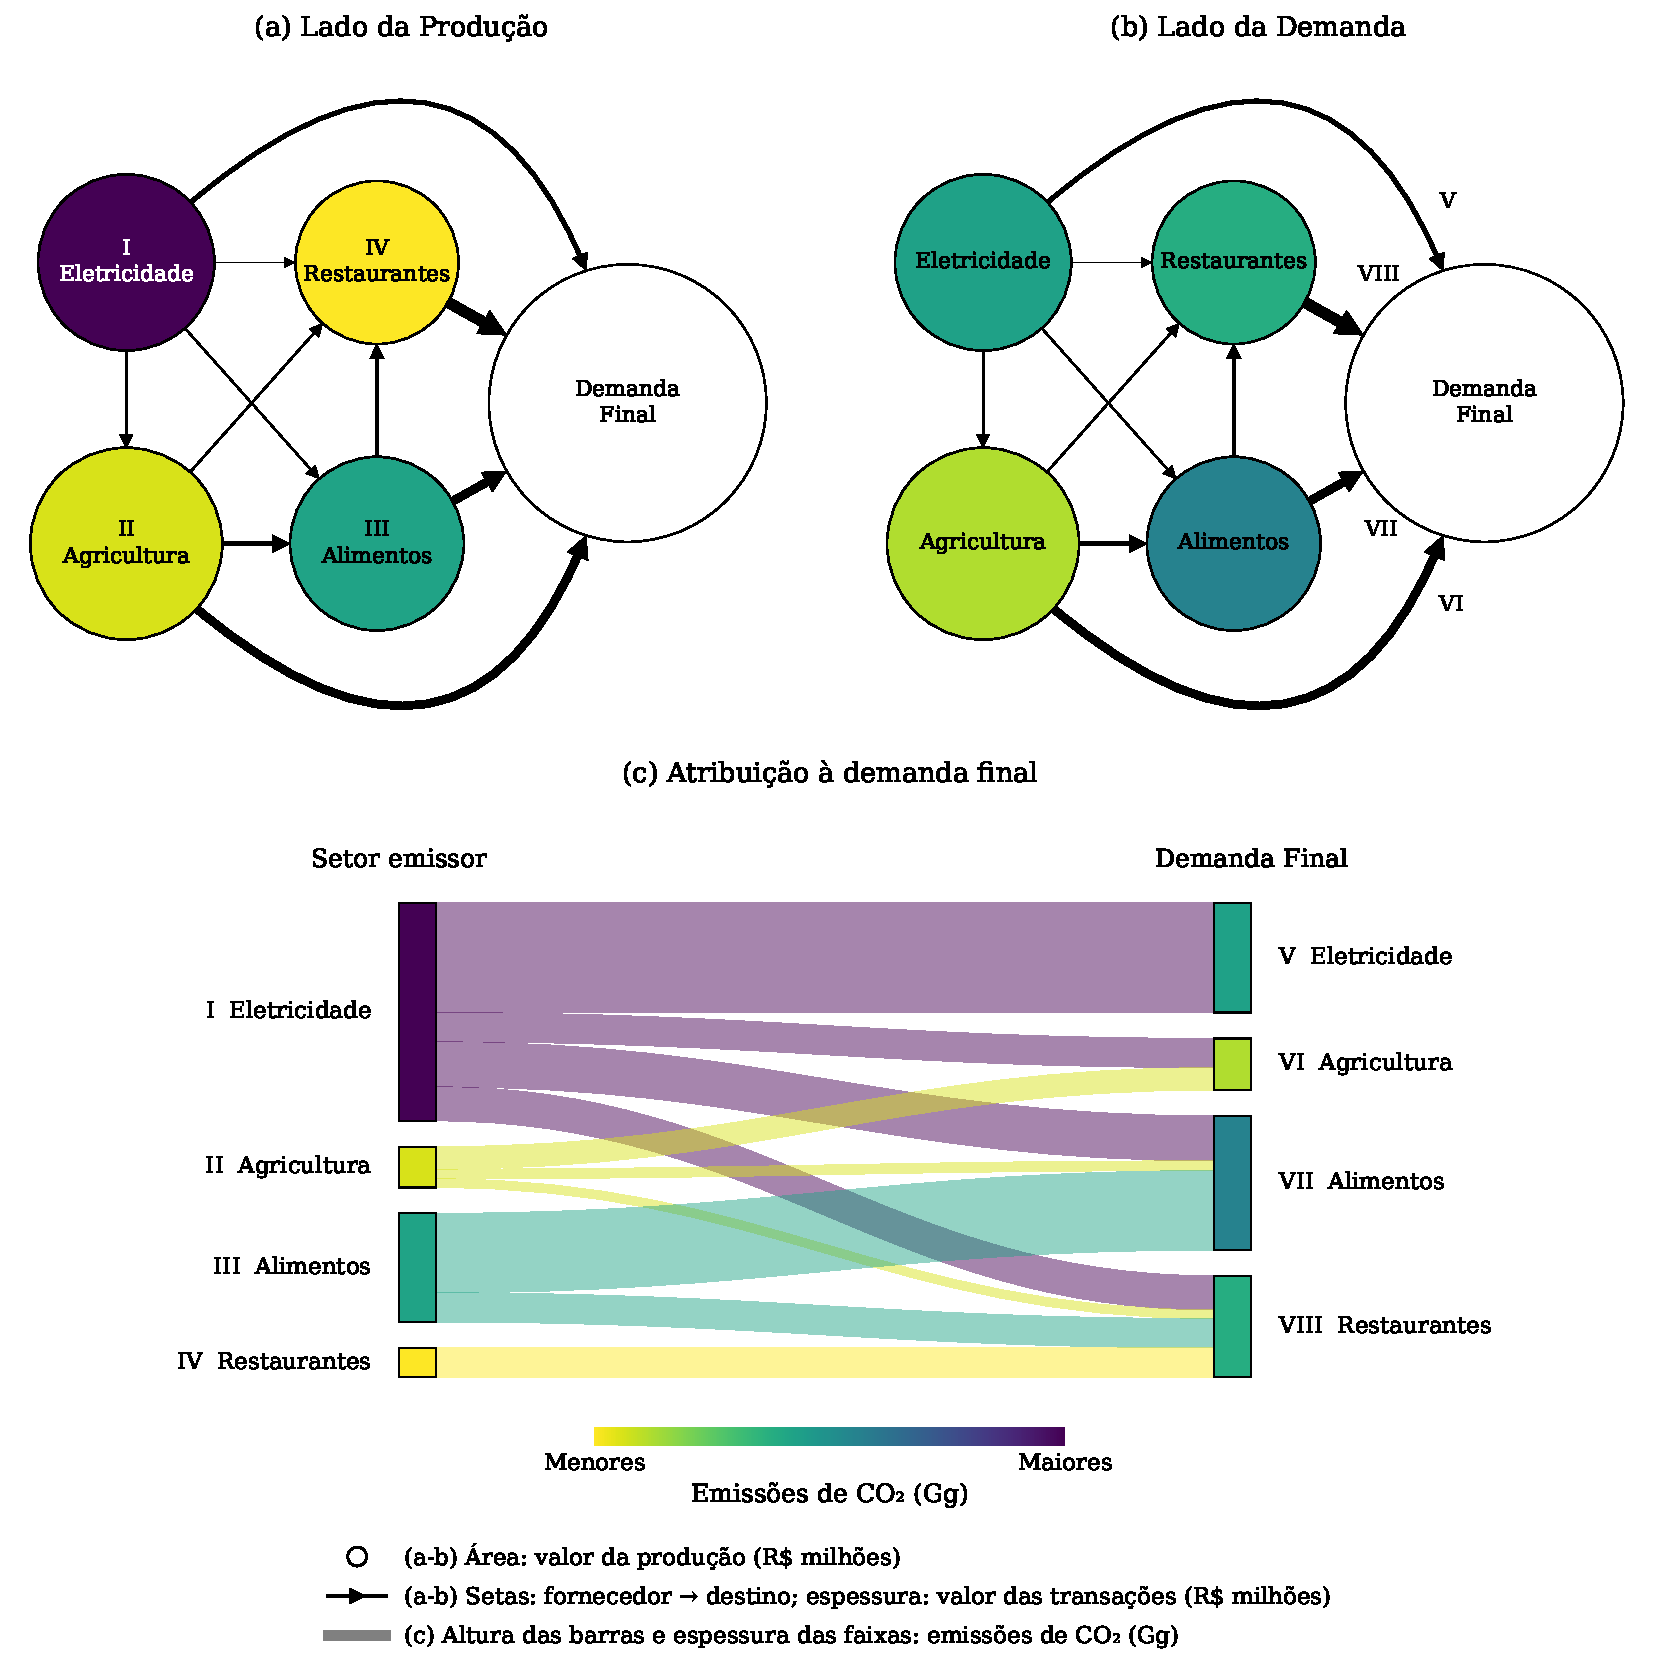
\includegraphics[width=\textwidth,height=0.76\textheight,keepaspectratio]{figuras/atribuicao_cadeia_alimentos.pdf}
\caption{Atribuição das emissões pela produção e pela demanda em uma economia ilustrativa.}
\label{fig:exemplo-atribuicoes}
\begin{minipage}{\textwidth}\footnotesize
Fonte: elaboração própria.

Nota: exemplo didático, sem representar estimativas nacionais dos quatro setores. Em (a--b), áreas e espessuras das setas expressam valores monetários; no nó Demanda Final, a área indica o valor recebido, incluindo exportações. As cores representam $c$ em (a) e $u$ em (b). Em (c), as barras à esquerda representam as origens emissoras (I--IV) e as barras à direita, os produtos finais (V--VIII). Suas alturas e as espessuras das faixas expressam emissões em Gg de CO\textsubscript{2}. Os três quadros compartilham a escala de cores.
\end{minipage}
\end{figure}
\clearpage
